%The Materials and Methods section provides sufficient detail for other 
%scientists to reproduce the experiments presented in the paper. In some 
%journals, this information is placed in an appendix, because it is not what 
%most readers want to know first.

% explicit preview would be phrased much like the object of the document: 
%"This section first . . . , then . . . , and finally . . . "
% Do not make readers guess: Make sure the paragraph's first sentence gives 
%them a clear idea of what the entire paragraph is about.
%%%%%%%%%%%%%%%%%%%%%%%%%%%%%%%%%%%%%%%%%%%%%%%%%%%%%%%%%%%%%%%%%%%%%%%%%%%%%%
\section{Adaptive Optics Methods applied in Microscopy}
\label{sec:ExperimentDiscussion}

AO has been demonstrated in a range of microscope modalities, including 
conventional widefield microscopes as well as laser scanning systems. The 
most common implementations have involved confocal and two-photon 
fluorescence microscopy, both of which are widely used methods in biomedical 
investigations. Due to aberrations, these microscopes suffer from a 
significant drop in signal and resolution as the focus is moved deeper into 
the specimen. 

Various research groups have combined these microscopes with direct wavefront 
sensing and sensorless AO, normally using deformable mirrors for aberration 
compensation. Ji et al. developed another approach that uses an SLM to 
implement a pupil segmentation phasing method in a two-photon microscope. AO 
has also been applied to microscopes using more exotic contrast mechanisms 
based upon nonlinear optical processes, such as second- and third-harmonic 
generation or coherent anti-Stokes Raman scattering. Using these various 
methods, researchers have demonstrated image improvement at depths of up to 
100 ìm in mouse embryos and over 200 ìm in brain tissue.

Adaptive microscopy is also finding a role in the imaging of live specimens. 
It can help to reduce the time required for image acquisition by increasing 
signal generation and collection efficiency. This is particularly useful in 
microscopes that rely on nonlinear contrast mechanisms, where any drop in 
focal intensity has a compounded effect on signal level.

AO can help by allowing the designer to relax the aberration tolerance from 
the usual fraction of a wavelength up to several wavelengths. This permits a 
significant reduction in the complexity of the optical system. In 
configurations where the optical fidelity has been compromised, the AO can be 
used to correct the residual system aberration, restoring diffractionlimited 
operation.

% explain that we need AO, ref this:
We can conclude: specimen induced aberrations lead to reduced signal levels 
and a deterioration in image quality in optical microscopy, especially in CFM 
and TPM. For the first time, specimen induced aberrations that occur with 
various biological specimens have been classified and quantified for the most 
relevant condition of high NA. The above approach can provide detailed 
information about the variation of each Zernike coefficient across the scan.
As expected from theory, lower NA systems are less susceptible to aberrations 
than high NA system under otherwise similar conditions. Low order correction 
would still provide benefits, even though the initial aberrations are 
smaller. The results presented here quantify the benefit of adaptive optics 
for biological microscopy and provide the bounds within which these systems 
must operate.
\cite{characterizing_abberations}

%%%%%%%%%%%%%%%%%%%%%%%%%%%%%%%%%%%%%%%%%%%%%%%%%%%%%%%%%%%%%%%%%%%%%%%%%%%%%
\subsection{Widefield Microscopy}
\label{sec:WidefieldMicroscopy}

In conventional microscopes, widefield illumination is provided using either 
transmission optics or, in the case of re ection or uorescence modes, via the 
objective lens in an epi configuration. In either case, the image quality 
depends only on the optics of the detection path and is independent of the 
fidelity of the illumination path.
Aberration correction is therefore only necessary in the detection path and a 
single pass adaptive optics system will suffice.
\cite{Aberrations_book} 

The objective of all adaptive optics systems is to reduce the wave front 
aberrations to an acceptable level. Normally this would involve a wave front 
sensor to measure the aberrations, which are in turn corrected using an 
adaptive element, such as a deformable mirror. In imaging systems, however, 
direct wave front sensing is not straightforward and wave front sensorless 
schemes are often employed. In certain situations, some aberration 
information can be extracted from a single image using phase retrieval 
methods; further information is obtained from two or more defocused images 
using the methods of phase diversity.


%------------------------------------------------------------------------------
\subsubsection{Transmission Microscope}
\label{sec:TransmissionMicroscope}
all from \cite{wide_AOM_loew_freq} which \cite{wide_AOM_structured_illu} is based on, i.e. where it is the more advandced topic

%basic principle:
- arbitrary induced aberrations
- find a metric whit which one can measure the aberrations of the single 
modes and that can be easily optimized
- metric based on modes which need to be independent -> Zernike or Luzkov can 
be used
- certain spatial frequency range is picked (low spatial frequency required) 
- metric provides max. at the value of the coefficient for the mode chosen, 
see figure???
- by introducing 3 artificial aberrations (0, +- bias) the max of the 
lorentzian function can be found readily!


Aberration correction is performed through the optimisation of an image 
quality metric based upon the low spatial frequency content of the image. A 
sequence of images is acquired, each with a different aberration bias applied 
and the correction aberration is estimated from the information in this image 
sequence. It is shown, by representing aberrations as an expansion in Lukosz 
modes, that the effects of different modes can be separated. The optimisation 
of each mode becomes independent and can be performed as the maximisation of 
a quadratic function, requiring only three image measurements per mode. This 
efficient correction scheme is demonstrated experimentally in an incoherent 
transmission microscope. We show that the sensitivity to different aberration 
magnitudes can be tuned by changing the range of spatial frequencies used in 
the metric.We also explain how the optimisation scheme is related to other 
methods that use image sharpness metrics.

By using knowledge of the maximised function’s topology, we were able to 
optimise algorithms to provide higher efficiency. The results indicated that 
deterministic, non-adaptive algorithms could be effective in controlling 
these systems, if suitably formulated. We demonstrated the relative 
effectiveness of the different algorithms as the number of aberration modes, $
N$, was increased. The number of measurements required in other methods 
increased quadratically or  exponentially with $N$~\cite{wide_sphere_packing}
The direct maximisation method was significantly more efficient, requiring 
only $N+1$ measurements for $N$ modes, over the range of input aberrations 
used here. This improvement over the other methods was possible since the 
calculation effectively took into account a priori knowledge about the form 
of the function being maximized. This is applicable to any system where the 
aberration can be accurately represented by the N orthonormal modes.

Certain adaptive optics systems do not employ a wave front sensor but rather 
maximize a photodetector signal by appropriate control of an adaptive 
element. The maximization procedure must be optimized if the system is to 
work efficiently. Such optimisation is often implemented empirically, but 
further insight can be obtained by using an appropriate mathematical model. 
In many practical systems aberrations can be accurately represented by a 
small number of modes of an orthogonal basis, such as the Zernike 
polynomials. By heuristic reasoning we develop a model for the operation of 
such systems and demonstrate a link with the geometrical problems of sphere 
packings and coverings. This approach aids the optimization of control 
algorithms and is illustrated by application to direct search and hill 
climbing algorithms. We develop an efficient scheme using a direct 
maximization calculation that permits the measurement of N Zernike modes with 
only N+1 intensity measurements.

These methods use iterative calculations based upon a model of the imaging 
process to retrieve the aberrations and the object structure. However, these 
calculations are not guaranteed to converge to a unique solution for 
arbitrary objects. In other wave front sensorless systems, the adaptive 
element is reconfigured in order to optimize a metric related to image 
quality. The optimization procedure involves measurement of the metric for a 
number of trial correction aberrations, followed by the estimation of an 
improved correction aberration. This process is repeated until the image 
quality is considered acceptable. The number of measurements required during 
this process depends upon the optimization algorithm and parameters used, the 
mathematical representation of the aberration, and the object structure. An 
effective model-based adaptive optics scheme should be object independent, so 
the model should permit the separation of aberration and object influences on 
the measurements.We show that this separation is possible through the 
appropriate choice of optimization metric and aberration representation

In this paper we describe and demonstrate an image-based adaptive optics 
scheme that is predominantly independent of object structure. This scheme 
uses the low spatial frequency content of the image as the optimisation 
metric but leads to correction for all spatial frequencies. The aberration is 
represented in terms of Lukosz modes~\cite{wide_Lukosz_Modes}; these modes 
are ideal for modelling the effects of aberrations on the imaging of low 
spatial frequencies . We describe the imaging process in terms of spectral 
densities and the optical transfer function. The optimisation metric g is 
introduced as the sum of a range of low frequencies and is related to the 
coefficients of the aberration expansion, {ai}. Because of this choice of 
aberration expansion and optimisation metric, the function g({ai}) is found 
to have a paraboloidal maximum that permits the use of simple maximisation 
algorithms. Moreover, we show that this optimisation can be performed as a 
sequence of independent maximisations in each aberration coefficient. The 
correction scheme is demonstrated for imaging in an incoherent transmission 
microscope.

In order to understand the effects of the aberration on I 1, it is useful to 
represent the aberration as a combination of Lukosz functions. These 
functions, based upon the Zernike polynomials, were first derived by Lukosz [
14] and later, independently by Braat [15]. Like Zernike circle functions, 
the Lukosz functions are each expressed as the product of a radial polynomial 
and an azimuthal function and use the same dual index and numbering scheme. 
They can be defined as

we optimize the energy within a certain frequency range ? 

the value of ak that minimises G(ak) can be calculated from a minimum of 
three measurements of G. In practice, we took these three measurements by 
intentionally introducing different aberrations using the adaptive element. 
We refer to these aberrations as biases.

An image was acquired and its FT and spectral density were calculated. The 
appropriate range of frequency components was summed, giving the metric 
measurements g-, g0 and g+ respectively, and the reciprocal of each result 
was calculated, giving G-, G0 and G+. The optimum correction aberration was 
then estimated by parabolic minimisation as~\cite{wide_parabolic_optimization}
...

\begin{align}
	a_\text{corr} = \frac{b(G_+ - G_-)}{2G_+ - 4G_0 + 2G_-}
\end{align}

which is exactly equivalent to the Lorentzian maximisation of the metric g. 
To correct this single mode, the correction aberration $\Phi = a_\text{corr}L_
k$ would be added to the deformable mirror. For multiple mode correction, 
each modal coefficient would be measured in this manner before applying the 
full correction aberration containing all modes.

The correction process is illustrated in Fig. 4 for the correction of one 
Lukosz mode using the scatterer specimen. A suitable range of spatial 
frequencies and the bias amplitude were chosen based upon the curves in Fig. 3
. An initial aberration was added using the DM, an image was acquired and the 
value of g was calculated. Positive and negative bias aberrations were added 
in turn and the corresponding values of g were calculated. The correction 
aberration was obtained using Eq. 33 and the correction was applied to the DM.

However, in all cases shown here, this corresponds to a Strehl ratio of 
greater than 0.8, close to the diffraction limit. These results indicate 
that, when aberration statistics are unknown, a sensible strategy would 
involve choosing small spatial frequencies for an initial correction. This 
would be accompanied by a bias that is no larger than the half width of the 
response curve, as shown in Fig. 3(b). If further correction is required, 
this could be performed using a larger range of frequencies and a 
corresponding smaller bias. If the maximum expected aberration magnitude is 
known, then the bias could be chosen to be similar to this maximum. 

The effect of additional aberration modes on the correction process was investigated by including random combinations of an extra eight modes (i = 12 to 19) in the initial aberration. The original eight modes (i = 4 to 11) were corrected in the same manner as before and å was calculated taking into account only the modes that were corrected. The results obtained when different amounts of the additional modes were present are shown in Fig. 7. The error å shows only a small variation as the amplitude ofk the additional modes is increased. This illustrates that different aberration modes can be corrected independently using this procedure.

We have introduced a model-based adaptive optics scheme for correcting aberrations in an incoherent imaging system. Using an optimisation metric based upon the low spatial frequency content of the image and an aberration expansion in terms of Lukosz modes, we have been able to separate the effects of the different aberration modes. This allowed the optimisation to be performed as a sequence of independent corrections of each mode. Although only low spatial frequencies are used in the optimisation process, correction of all aberrations (aside from piston, tip and tilt) results. Consequently, imaging quality is improved for all spatial frequencies and not solely the frequencies used in the optimisation metric. The correction scheme is predominantly independent of object structure – the model is valid when the low spatial frequency components are not significantly concentrated in one orientation. This would occur, for example, if the image were dominated by a one dimensional grid-like pattern. Even if the object has this form, we expect the scheme to be robust – this has been indicated by preliminary results. Although the discussion in this paper was framed in the context of an incoherent imaging system, we expect this approach also to be valid for coherent or partially coherent systems.
 

\begin{figure}[tbh]
        \centering
        \begin{subfigure}[b]{0.8\textwidth}
                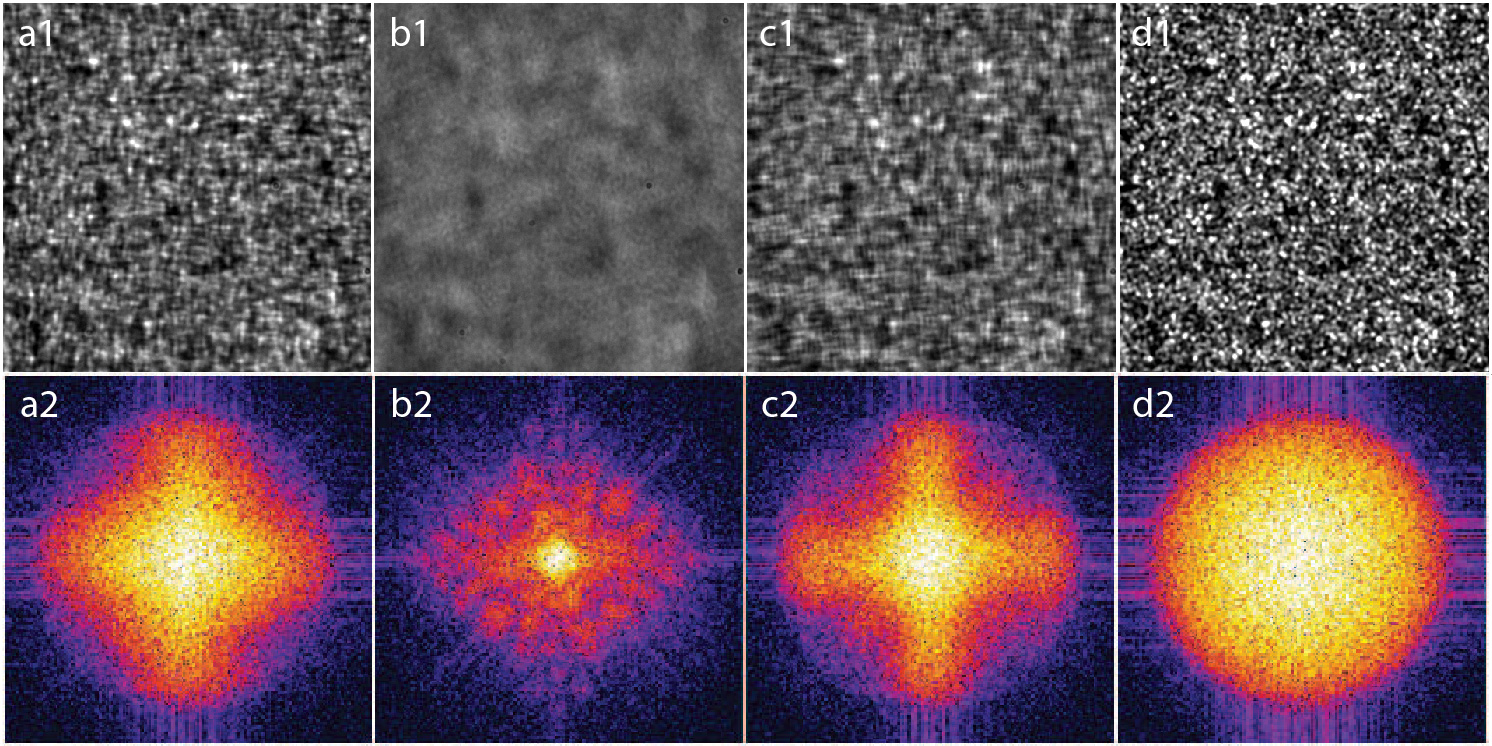
\includegraphics[width=\textwidth]{images/wide_parabolic_opti_images}
                \label{fig:para_opt_images}
        \end{subfigure}
        \begin{subfigure}[b]{0.8\textwidth}
                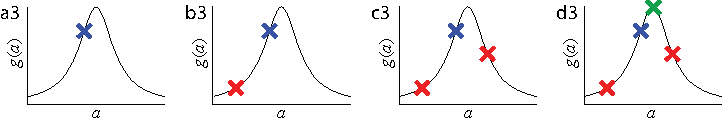
\includegraphics[width=\textwidth]{images/wide_parabolic_opti_graphs}
                \label{fig:para_opt_graphs}
        \end{subfigure}								
        \caption{Correction of a single Lukosz aberration mode (astigmatism, i = 5) for a scatterer specimen and using low spatial frequencies. The first row shows the raw images of the specimen and the second row contains the corresponding spectral densities. The third row illustrates schematically the sampling of the Lorentzian curve used in the optimization calculation. (a1-a3) correspond to an arbitrary initial aberration of magnitude, (b1-b3) have an additional negative bias while (c1-c3) have an additional positive bias of equal magnitude. (d1- d3) show the corrected image calculated with the parabolic minimizationn. Image after~\cite{wide_AOM_loew_freq}.
.}
\label{fig:para_opt}
\end{figure} 


%------------------------------------------------------------------------------
\subsubsection{Structured Illumination Microscopy}
\label{sec:StructuredIlluminationMicroscopy}

%next part all from
\cite{wide_AOM_structured_illu}

Optical sectioning microscopy is widely used to provide three-dimensional 
fluorescence images of biological specimens. A common way of obtaining this 
sectioning ability is through point scanning methods such as confocal or 
multiphoton microscopy [1, 2]. An alternative is to use a wide-field 
technique such as structured illumination (SI) microscopy, which retains the 
sectioning ability of confocal microscopy, but can be implemented in a 
conventional microscope using an incoherent light source, and without the 
need for scanning. 

In this technique, the image of a grid is projected on the specimen so as to 
produce a one-dimensional sinusoidal excitation pattern in the focal plane of 
the objective lens. The resulting fluorescence image, consisting of both in-
focus and out-of-focus fluorescence emission, is acquired by a camera. 
Several images are taken, each corresponding to a different grid position. As 
the grid pattern appears only in the focal plane, it is possible to extract 
an optical section from the spatially modulated component of the images via a 
simple calculation.~\cite{wide_structured_illu_principle}.

In this paper we describe wavefront sensorless adaptive optics implemented in 
a SI microscope. It is shown that the final image quality depends 
predominantly on the imaging efficiency of the illumination pattern’s spatial 
frequency. This imaging efficiency is affected much more by some aberration 
modes than by others. Consequently, different aberration modes can have 
significantly different effects on the final sectioned image.

The SI microscope relies upon the projection of a physical grid pattern into 
the focal plane of the specimen. We assume that the grid object is a 
sinusoidal transmission mask

those aberrations that affect the grid frequency have the most significant 
effect on the SI microscope. It is therefore useful to separate aberration 
modes into two groups: those that affect the grid frequency (referred to 
hereon as “grid modes”) and those that have no influence on this frequency (
“non-grid modes”). It is clear that grid modes have a significant influence 
on the intensity of the sectioned image, whereas non-grid modes have 
comparatively little effect. The non-grid modes do however affect the 
resolution.

%3. Derivation of a general optimisation scheme 
The specification of a modal aberration correction scheme requires the choice 
of three components: the aberration representation (the mathematical 
functions used to describe the aberrations), the optimisation metric (a 
quantity representing the image quality) and the estimator (the algorithm for 
estimating the correction aberration).

We would like to choose a metric function M whose maximum corresponds to the 
highest quality image.
find an aberration expansion for which the modes act independently on the 
metric.
This would allow the independent optimisation of each mode.
When M is expressed in this form, it is clear that independent maximisation 
with respect to each xi is possible. Furthermore, as the function is 
quadratic, the maximum can be found directly from three measurements of M 
corresponding to three different values of xi - here they reference to \cite{
wide_AOM_loew_freq} so maybe I should put the two together, or see this one 
as a more advandced version of the previous
\begin{align}
	M = M_0 - \sum_i{x_i^2}
	\label{eq:structured_metric}
\end{align}
In practice, these measurements would be taken with three different trial 
aberrations introduced by the correction element. However, M only takes the 
form shown in Eq.~\eqref{eq:structured_metric} if the aberration 
representation is appropriately chosen. 

for each aberration mode, the metric M was measured when adding a given 
amount of the considered mode, then again when substracting the same amount. 
Along with the measured value of M when no aberration was added, this allowed 
us to estimate the initial aberration present in each of the assessed modes 
and hence to correct these aberrations

Here we want to emphasise that the use of the appropriate metric and 
aberration modes means that the correction of N modes was performed using 
only 2N+1 measurements, thereby minimizing the increase in illumination time 
of the sample required for the correction.

The acquisition time per sectioned image was 300-500ms and the total time 
required for correction of 11 modes was 7-12s, depending on the sample.


However, M only takes the form shown in Eq. ( 10) if the aberration 
representation is appropriately chosen.


We are therefore led to the conclusion that the SI microscope, in comparison 
to other sectioning microscopes, is more susceptible to certain aberrations (
grid modes) and more resilient to others (non-grid modes).

Whilst the SI microscope relies upon a relatively simple optical principle, 
the image formation process has a complex mathematical description. 
Similarly, the derivation of a modelbased, sensorless, adaptive optical 
scheme is a complex process. However, our results show that the scheme is 
effective in correcting specimen-induced and system aberrations and restoring 
image quality. For the samples presented here, we found that the aberration 
mainly consisted of astigmatism, coma and spherical aberration modes.

The adaptive scheme described here has significant advantages over model-free 
algorithms in that the aberration correction can be estimated using a small 
number of measurements (2N+1 for N aberration modes). Moreover, as the scheme 
is mostly independent of the object structure, the appropriate modes have 
only to be determined once and the same scheme can be used for any 
specimen.We have also shown that aberration correction can be effectively 
combined with background subtraction to further improve SI microscope images. 
In the results presented here, aberration correction was performed as an 
average over an image frame and therefore would not correct for any local 
variations in aberrations. If these variations were found to be significant, 
the image could be formed from several sub-images for which independent 
aberration correction would be performed.

We have presented a general method that provides an optimal aberration 
expansion for a chosen optimisation metric. This relied upon the derivation 
of an inner product from a mathematical model of the imaging process, 
followed by an orthogonalisation process applied to a set of basis functions, 
such as the Zernike functions. This process reveals a wealth of information 
about the effects of different aberration modes on an imaging system – for 
the SI microscope, it enabled us to derive the sets of grid modes and non-
grid modes. \textbf{This method could equally be applied to any sectioning 
microscope to derive aberration expansions that are best suited to that 
application.
}
\begin{figure}
	\centering
		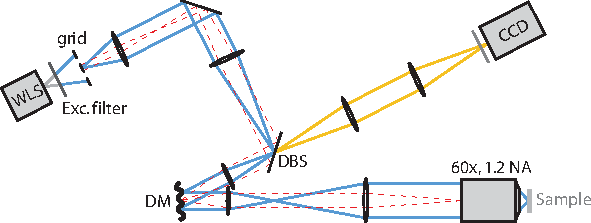
\includegraphics[width=0.75\textwidth]{images/wide_structured_illumination.pdf}
	\caption{Experimental setup for structured illumination microscopy with 
aberration correction. WLS~-~white light source, DM~-~deformable mirror, DBS
~-~dichroic beamsplitter. The blue rays mark the illumination path; the 
detection path is shown in yellow. Image after~\cite{wide_AOM_structured_illu}
.}
	\label{fig:wide_structured_illumination}
\end{figure}

\begin{figure}[tbh]
        \centering
        \begin{subfigure}[b]{0.3\textwidth}
                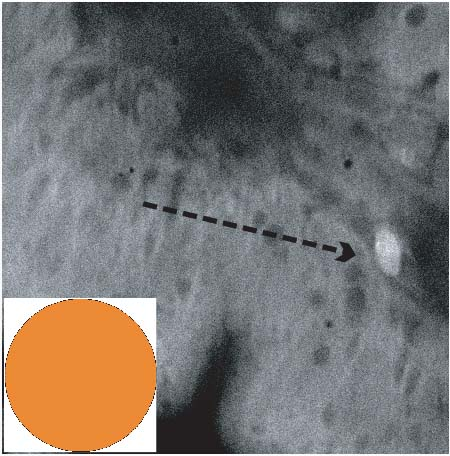
\includegraphics[width=\textwidth]{images/structured_illumination_uncorrected}
                \caption{Uncorrected.}
                \label{fig:SI_uncorrected}
        \end{subfigure}
        \begin{subfigure}[b]{0.3\textwidth}
                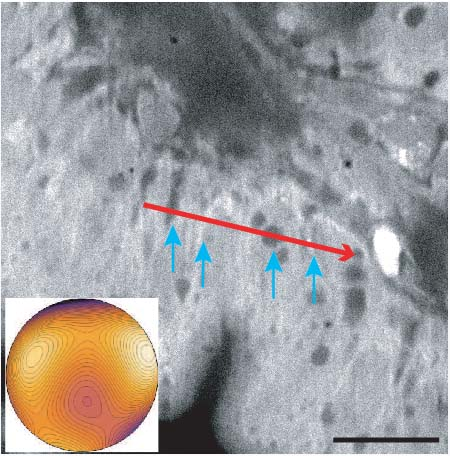
\includegraphics[width=\textwidth]{images/structured_illumination_corrected}
                \caption{Corrected.}
                \label{fig:SI_corrected}
        \end{subfigure}
        \begin{subfigure}[b]{0.3\textwidth}
                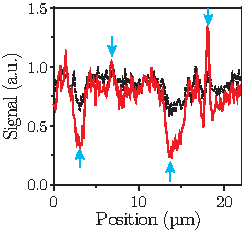
\includegraphics[width=\textwidth]{images/structured_illumination_scan}
                \caption{Line Scan.}
                \label{fig:SI_scan}
        \end{subfigure}
								
        \caption{Aberration correction in structured illumination microscopy. 
A fluorescent mouse intestine sample was imaged (a) without (b) with 
aberration correction with inserts showing the phase induced by the 
deformable mirror. (c) Profile along the lines drawn on the images, both 
profiles normalized so that their mean value is identical. As a result of the 
resolution improvement, the contrast of small sample features (blue arrows) 
are better defined after (red solid line) rather than before (black dotted 
line) correction. The imaging depth was approximately $\unit[10]{\upmu}$, 
sacle bar size $\unit[10]{\upmu}$. Image after~\cite{wide_AOM_structured_illu}
.}
\label{fig:structured_light_correction}
\end{figure} 

%------------------------------------------------------------------------------
\subsubsection{Fluorescence Microscopy}
\label{sec:FlourescnecMicroscopy}

next section, all from \cite{wide_AOM_FM_spehrical_correction} uses a 
standard widefield flourescene microscope but use AOM to correct for 
spherical aberration due to depth -> no specimen induce correction
uses deconvolution to get out of foucs photons corrected

In this paper, we concentrate on the depth dependent aberration which can 
quickly become serious. Imaging 20 mum a live sample (index of refraction 1.36
) with an oil immersion lens causes the peak intensity of the point spread 
function (PSF) to drop 3-fold and the width of the PSF in the axial direction 
to increase by 2-folds. \cite{wide_AOM_FM_spehrical_correction} 

Because wide-field microscopy captures as efficiently as possible every 
emitted photon ultimately minimizing the sample excitation dose, it is well 
suited to in vivo imaging in sampleswhere scattering is not too large. 
Although the out-of-focus photons are in thewrong place, they can be 
effectively re-assigned to the location of emission by constrained 
deconvolution algorithms \cite{wide_deconvolution}

The problem of depth aberrations can be solved by matching the sample index 
and the index of the immersion medium, but this is frequently not feasible or 
desirable. For example, the index of fixed cells can be matched to that of 
the immersion oil, but this option is not available for live imaging.

An important drawback to most schemes that have been proposed so far is that 
they require several images to be taken to optimize the aberration 
correction. This presents a serious problem for live imaging in biology 
because the fluorescence intensities can be weak and susceptible to rapid 
bleaching.

The approach we follow is to correct the depth aberrations withanopen-loop 
predictive algorithm similar totheapproach taken by Potsaid et al. in 
correcting off-axis aberrations. This is possible because the depth 
aberration can be calculated for a given depth into the sample. The depth 
aberration is the result of depth-dependent path length differences.

Correcting depth aberrations with a DM improves both the peak intensities and 
the deconvolution of images taken below the cover slip by removing the depth 
aberration. This allows the use of fast space-invariant deconvolution 
algorithms instead of depth-dependent algorithms. This is significant because 
it improves both the signal-to-noise ratio and the resolution in biological 
imaging where photons are in short supply. Unfortunately, the performance 
does not yet achieve what is theoretically possible.

\begin{figure}[htb]
	\centering
		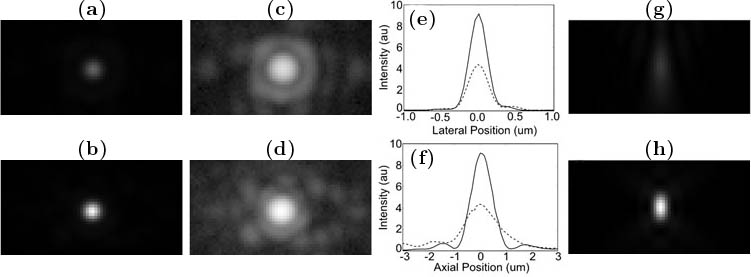
\includegraphics[width=0.80\textwidth]{images/wide_flour_spher_All.jpg}
	\caption{Images of a $\unit[200]{nm}$ bead $\unit[67]{\upmu m}$ below the 
cover slip in a water/glycerol mixture with n = 1.42.  (a) Uncorrected image 
of in-focus plane. (b) Corrected image of in-focus plane. Images (c) and (d) 
are the same as (a) and (b), respectively, but on a logarithmic scale for 
better visualization. (e) and (f) are line profiles of the intensity through 
the center of the bead along the lateral and the longitudinal axis, 
respectively. The dashed line is from the uncorrected image and the solid 
line is from the corrected image. (g) and (h) are simulations of the PSF. 
Images based on \cite{wide_AOM_FM_spehrical_correction}.}
	\label{fig:wide_flour_spher_All} 
\end{figure}


The first is the effect of uncorrected aberrations from the sample and the 
optical path, which decrease the maximum intensity at the cover slip, but in 
a way that does not add linearly to the depth aberration. Thus only a 
fraction of the dispersed photons can be restored to the central peak. In 
closed loop AO systems, system aberrations are automatically compensated at 
each position (Wright et al., 2007), but in an open-loop system this is not 
possible. The second factor is the inability of the mirror to precisely 
conform to the shape given by Eq. (1). The residual error of the mirror shape 
increases with depth (see Fig. 3c) so that as the imaging plane goes deeper 
and the possibility for improvement becomes greater, the improvement in peak 
intensities decreases

Lastly, the ultimate goal of applying adaptive optics in microscopy is to 
correct all aberrations including those introduced by the refractive index 
variations of the sample itself.
\cite{wide_AOM_FM_spehrical_correction}

\cite{wide_MPFM}


%------------------------------------------------------------------------------
-
\subsection{Point Scanning Microscopes}
\label{sec:PointScanningMicroscopes}

Scanning optical microscopes are widely used for high resolution imaging, 
mainly because certain implementations provide three-dimensional resolution 
with optical sectioning and are thus particularly useful for imaging the 
volume structures of biological specimensz. In these microscopes, 
illumination is provided by a laser that is focused by an objective lens into 
the specimen. The light emitted from the specimen is collected, usually 
through the same objective lens, and its intensity is measured by a single 
photodetector. The focal spot is scanned through the specimen in a raster 
pattern and the image is acquired in a point-by-point fashion. The resulting 
data are stored and rendered as images in a computer.

Several other point scanning microscope modalities have been introduced, 
including two-photon excitation uorescence (TPEF) microscopy, second harmonic 
generation (SHG) and third harmonic generation (THG) microscopy, and coherent 
anti-Stokes Raman (CARS) microscopy.

%------------------------------------------------------------------------------
-
\subsubsection{Confocal Microscopes}
\label{sec:ConfocalMicroscopes}

The most common example of this type is the confocal microscope, which can be 
operated in reflection or fluorescence mode. Three-dimensional resolution is 
achieved by the placement of a pinhole in front of the photodetector. In a 
reflection mode confocal microscope, the illumination is scattered by objects 
not only in the focal region, but throughout the focusing cone. In 
fluorescence mode, emission is generated in the focus but also in out-of-
focus regions. The pinhole ensures that mainly light from the focal region 
falls upon the detector and light from out-of-focus planes is obscured. It is 
critical in the confocal microscope that both the illumination and detection 
paths are diffraction limited. This ensures that i) the illuminating focal 
spot is as small as possible, and ii) that the focus is perfectly imaged on 
to the detector pinhole. Therefore, in an adaptive confocal microscope, 
aberration correction must be included in both paths. This dual pass adaptive 
system can usually be implemented using a single deformable mirror, if the 
path length aberrations are the same for both the illumination and the 
emission light. This is the case if there is no significant dispersion in the 
specimen or chromatic aberration in the optics.

A pinhole is not required to obtain three-dimensional resolution, so most 
TPEF microscopes use large area detectors to maximise signal collection. 
Although they rely upon other physical processes, non-linear imaging 
modalities such as SHG, THG and CARS exhibit similar resolution properties. 
When using large area detectors, the fidelity of imaging in the detection 
path is unimportant so the effects of any aberrations in this path are 
negated. It follows that single pass adaptive optics is appropriate for these 
microscopes as aberration correction need only be implemented in the 
illumination path.

Adaptive optics systems have been successfully combined with several point-
scanning microscope systems including confocal,13 TPEF,6, 14, 15 harmonic 
generation,16, 17 CARS.18 Example images of aberration correction in an 
adaptive THG microscope are shown in Fig. 10.

\cite{book_confocal}
\cite{AOM_scan_CFM}


%------------------------------------------------------------------------------
-
\subsubsection{Two-Photon Fluorescence Microscopy}
\label{sec:twoPhotonExcitation}

\cite{TPFM_gated_wavefront}
\cite{TPFM_image_based}
\cite{TPFM_pratical}

%------------------------------------------------------------------------------
-
\subsubsection{Harmonic Generation}
\label{sec:HarmonicGeneration}

\cite{HG_embryos}
\cite{HG_dynamic}


%------------------------------------------------------------------------------
-
\subsubsection{CARS}
\label{sec:CARS}

\cite{CARS}



